\documentclass[10pt]{article}
\usepackage[margin=0.9in]{geometry}
\usepackage{graphicx}
\usepackage{booktabs}
\usepackage{amsmath}
\usepackage{caption}
\usepackage{subcaption}
\usepackage[hidelinks]{hyperref}
\usepackage{float}
\captionsetup{font=small}
\setlength{\parskip}{4pt}
\setlength{\parindent}{0pt}

\title{\vspace{-2.5em}Improving the Deep Detector on FLAME-3:\\
A Diagnosis-Driven Investigation}
\author{CS269 Project --- Deformable Models}
\date{\today}

\begin{document}
\maketitle
\vspace{-1.5em}

\section{Starting Point and Question}

In the baseline study, segmenting the thermal-defined fire ($\ge150\,^\circ$C) from
RGB-only input proved hard: the color floor scored IoU $0.004$ (the fire is
smoke-obscured, no redder than background), oracle-initialised contours reached
$0.365$ but only by \emph{refining a handed-in location}, and a from-scratch
U-Net---the best honest, prior-free detector---plateaued at \textbf{IoU 0.147}.
This report asks: \emph{can we improve the prior-free deep detector, and what is
actually limiting it?} We treat it as an inverse problem ($x$, the hot-region
support, recovered from RGB $y$ through a strongly smoothing smoke-occlusion
operator $A$) and test one change at a time against the 0.147 baseline, on the
same 94-frame test split, with identical IoU/Dice scoring.

The headline: four plausible improvements were essentially flat or negative; a
learning-curve diagnostic revealed the true bottleneck (\emph{data starvation});
and the fix that addressed it---augmentation, done correctly---gave the first
real gains, lifting U-Net to \textbf{IoU 0.179} ($+22\%$) and DALS to
\textbf{0.182} ($+49\%$), while leaving the detector-limited Deep Snake unmoved.
Figure~\ref{fig:score}
summarises every attempt; Table~\ref{tab:all} gives the full numbers and the
mechanism each intervention targeted.

\begin{table}[H]
\centering\small
\begin{tabular}{llrrl}
\toprule
Intervention & Lever & IoU & Dice & Verdict \\
\midrule
Color floor (reference) & none & 0.004 & 0.007 & trivial floor \\
U-Net \textbf{baseline} & --- & 0.147 & 0.207 & reference \\
Focal-Tversky loss & reweight data term & 0.153 & 0.221 & wash \\
\quad (DALS, same loss) & reweight data term & 0.115 & 0.172 & worse \\
$+R\!-\!G$ channel (4ch) & reparametrise input & 0.150 & 0.217 & wash \\
$+$HSV$+R\!-\!G$ (7ch) & reparametrise input & 0.135 & 0.193 & worse (overfit) \\
U-Net-seeded GAC & boundary refinement & 0.145 & 0.219 & no-op over detector \\
Thermal regression & restructure output & 0.068 & 0.111 & worse (harder target) \\
Strong aug, 50ep (U-Net) & synthetic data & 0.092 & 0.142 & confounded (under-trained) \\
\textbf{U-Net + medium aug, 120ep} & synthetic data & \textbf{0.179} & \textbf{0.247} & \textbf{win} ($+22\%$) \\
\textbf{DALS + medium aug, 120ep} & synthetic data & \textbf{0.182} & \textbf{0.254} & \textbf{best} ($+49\%$) \\
Deep Snake + medium aug, 120ep & synthetic data & 0.032 & 0.032 & flat (detector-limited) \\
\midrule
Oracle-GAC (\emph{not} prior-free) & location prior & 0.365 & 0.499 & upper reference \\
\bottomrule
\end{tabular}
\caption{Every intervention, grouped by the inverse-problem lever it pulls.
Only the lever that adds genuinely new information (synthetic data) beats the
baseline. All deep rows: 94-frame test split; contour rows: 592-frame set.}
\label{tab:all}
\end{table}

\paragraph{Inverse-problem reading.} Recovering $x$ from $y=A(x)$ when $A$ is
near-singular requires either (i) more measurements/data to constrain the fit,
or (ii) a prior that injects information $A$ destroyed. The oracle is route (ii)
in its purest form (the location is handed in), and it dominates. Among prior-free
methods, only route (i)---more effective data via augmentation---helped. Output-
and input-side reparametrisations (Focal-Tversky, channels, thermal regression)
change the \emph{form} of the problem without adding measurements or a genuine
prior, so the theory predicts, and the experiments confirm, that they cannot move
the achievable IoU.

\begin{figure}[H]
\centering
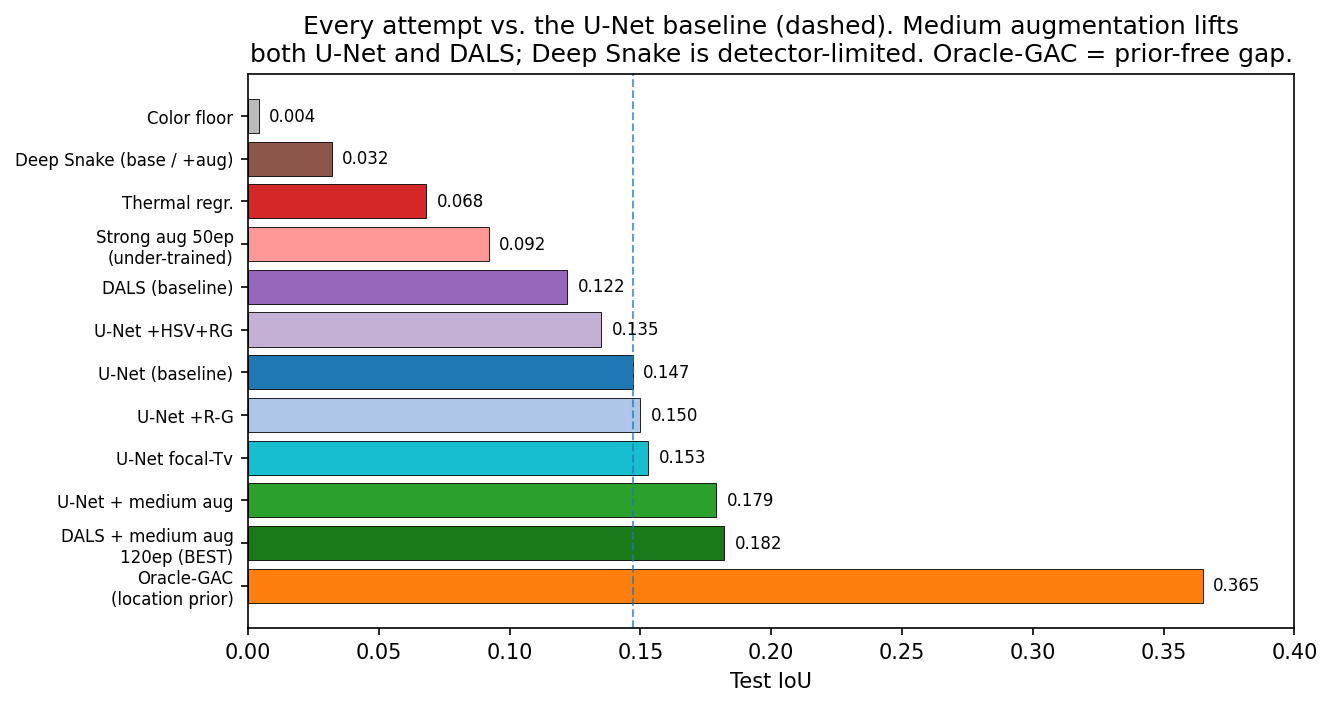
\includegraphics[width=0.85\textwidth]{figs/imp/scoreboard.png}
\caption{All attempts vs.\ the U-Net baseline (dashed). Oracle-GAC is shown only
to mark the prior-free gap; it is not prior-free.}
\label{fig:score}
\end{figure}

\section{Attempts That Did Not Help (and Why)}

\paragraph{(1) Focal-Tversky loss.} GT fire is $\sim$0.8\% of pixels and
fragmented (up to 67 components/frame), the regime where plain BCE+Dice
under-segments. We replaced it with Focal-Tversky ($\beta>\alpha$ penalises
false negatives harder). Result: U-Net $0.147\!\to\!0.153$, DALS
$0.122\!\to\!0.115$---a wash. Reweighting the data term cannot recover signal
that is not present.

\paragraph{(2) Engineered input channels.} We fed the classical $R\!-\!G$ fire
cue (and HSV) alongside RGB so the net need not rediscover it. Result: $+R\!-\!G$
$0.150$, $+$HSV$+R\!-\!G$ $0.135$ (\emph{worse}). A U-Net's first layer can
already form $R\!-\!G$ from RGB; the extra channels add no information, and the
7-channel input mildly overfits the small dataset.

\paragraph{(3) U-Net-seeded contour refinement.} Replacing the oracle/color init
of GAC with the U-Net prediction rescued the contour from total collapse
(color-init GAC $0.003 \to$ U-Net-init GAC $0.145$) but added \emph{nothing} over
the raw U-Net (0.147): the level set merely traces the mask it is given. Kass
fared worse (0.078)---a single closed contour cannot represent the fragmented
fire. \emph{The deformable model is a no-op refiner here; all the work is
detection.}

\paragraph{(4) Cross-modal thermal regression.} As an inverse-problem
regulariser we learned the structured intermediate $y\!\to\!\hat T$ (continuous
temperature) and thresholded at $150\,^\circ$C, hypothesising the dense graded
target would force the net to internalise $A^{-1}$. Result: \textbf{0.068},
well below baseline. Predicting temperature is strictly harder than predicting
the label and the threshold amplifies regression error; with limited data the
harder target hurts. A negative result, but an informative one.

\paragraph{Pattern.} Every lever that does not add \emph{new information}---loss
reweighting, input reparametrisation, output restructuring, boundary
refinement---is flat or negative. This motivated asking whether the limit is the
\emph{information} in the RGB or the \emph{amount of data}.

\section{Diagnosis: The Model Is Data-Starved}

We ran a learning curve: train the U-Net on 25/50/75/100\% of the 435 training
frames, with the validation set held \emph{fixed}, and record best val IoU
(Fig.~\ref{fig:lc}). The curve rises monotonically and \emph{is still climbing at
100\%} of the data ($+0.013$ over the last segment). A saturated,
information-limited model would have flattened. The signal \emph{is} in the RGB;
there are simply too few labelled frames---and they come from a handful of flight
runs, so the effective sample count is lower still---for a from-scratch U-Net to
extract it. This reframes the failed attempts: they did not fail because the task
is unsolvable, but because none of them addressed sample count.

\begin{figure}[H]
\centering
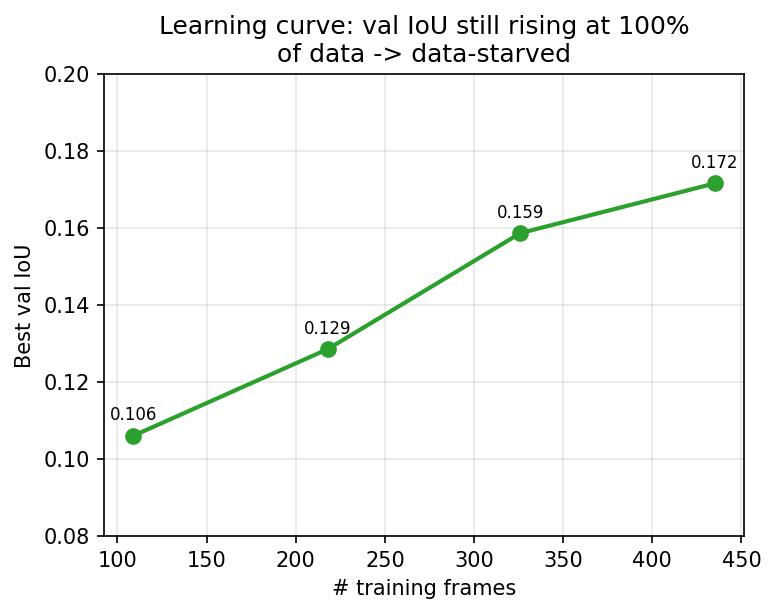
\includegraphics[width=0.5\textwidth]{figs/imp/learning_curve.png}
\caption{Best val IoU vs.\ training-set size (val fixed). Still rising at 100\%
$\Rightarrow$ data-starved: more data would help.}
\label{fig:lc}
\end{figure}

\section{The Fix: Augmentation, Done Correctly}

\paragraph{What ``augmentation'' means here.} All transforms operate on a
training pair (RGB image, binary mask). Geometric transforms are applied
\emph{identically} to image and mask so they stay co-registered (verified: a
synthetic aligned pair retains image/mask IoU $\approx0.99$ after augmentation);
photometric transforms touch the \emph{image only}, since the mask is a label,
not a brightness. We define three tiers (Table~\ref{tab:augtiers}):

\begin{table}[H]
\centering\small
\begin{tabular}{lll}
\toprule
Tier & Geometric & Photometric \\
\midrule
\textbf{light} (baseline) & horizontal flip ($p=0.5$) only & none \\
\textbf{medium} (the win) & flip; rotation $\pm10^\circ$; scale & brightness $\times[0.92,1.08]$; \\
 & $\times[0.95,1.10]$; shift $\pm4\%$ & contrast (additive $\pm8$); \emph{no hue} \\
\textbf{strong} & flip (H+V); rotation $\pm25^\circ$; scale & brightness/contrast; \\
 & $\times[0.85,1.20]$; shift $\pm8\%$ & \textbf{hue shift} $\pm8^\circ$ \\
\bottomrule
\end{tabular}
\caption{Augmentation tiers. \emph{light} = the original flip-only baseline.
\emph{strong} applies large warps and a hue shift; the latter is risky here
because the fire cue is a faint colour signal that hue rotation can destroy.
\emph{medium} keeps the geometry gentle and drops the hue shift.}
\label{tab:augtiers}
\end{table}

Geometric warps use reflection padding for the image and zero padding for the
mask; rotation/scale/shift are composed into a single affine so the image is
resampled once. Each is applied per sample at load time (online augmentation), so
every epoch sees a fresh random variant---the mechanism by which 435 frames
behave like a larger set.

Augmentation is synthetic data, so it should help a data-starved model---but our
\emph{first} attempt used the \emph{strong} tier at only 50 epochs and scored
\textbf{0.092}, worse than baseline. This was a confounded test, and the
confound is visible in the convergence curves (Fig.~\ref{fig:conv}): aggressive
augmentation slows convergence, and at a fixed 50-epoch budget the model was cut
off \emph{mid-climb}, not converged.

Removing both confounds---milder augmentation (flips, $\pm10^\circ$ rotation,
mild brightness/contrast, \emph{no} hue shift, which can destroy the faint fire
cue) and a longer 120-epoch budget---gives the first genuine improvement:
\textbf{test IoU 0.179, Dice 0.247}, a $+0.032$ ($+22\%$) gain over baseline.
The val curve climbs to $\sim$0.21 and converges, confirming the budget was
adequate.

\begin{figure}[H]
\centering
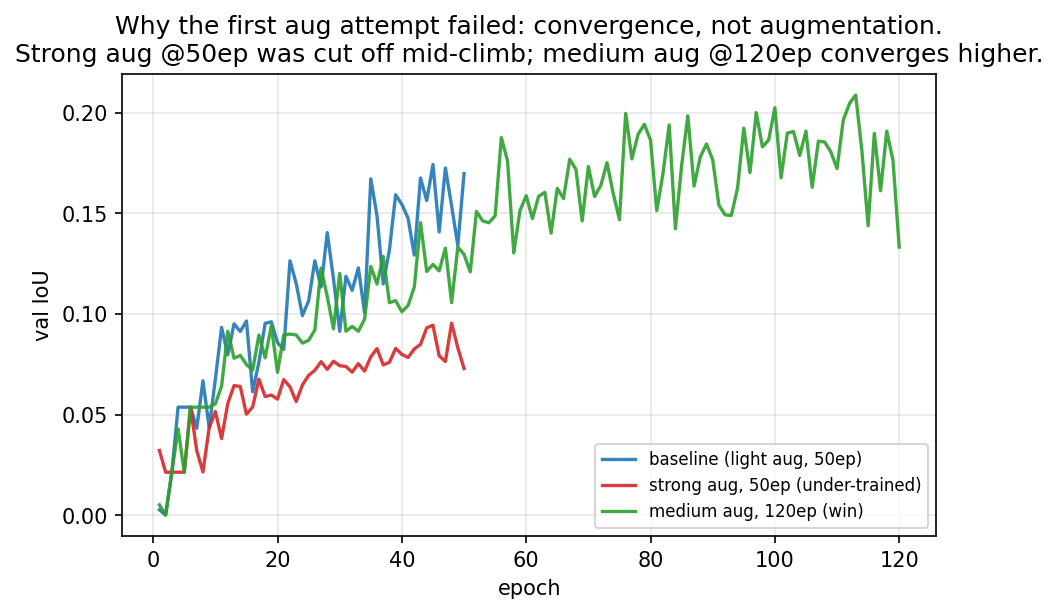
\includegraphics[width=0.7\textwidth]{figs/imp/convergence.png}
\caption{Validation IoU per epoch. The first augmentation attempt (red) was cut
off mid-climb at 50 epochs; the corrected run (green) converges higher than the
baseline (blue). The earlier ``augmentation hurts'' reading was a convergence
artifact.}
\label{fig:conv}
\end{figure}

\begin{table}[H]
\centering\small
\begin{tabular}{lrr}
\toprule
Run & Test IoU & Dice \\
\midrule
U-Net baseline (light aug, 50ep) & 0.147 & 0.207 \\
U-Net strong aug, 50ep (under-trained) & 0.092 & 0.142 \\
\textbf{U-Net medium aug, 120ep} & \textbf{0.179} & \textbf{0.247} \\
\bottomrule
\end{tabular}
\caption{The augmentation result, with the confounded intermediate run shown for
honesty.}
\label{tab:aug}
\end{table}

\paragraph{Does the fix transfer across architectures?} If data starvation is the
true bottleneck, the same augmentation should lift any architecture that can
\emph{use} the extra data. We retrained DALS and Deep Snake under the identical
protocol (medium aug, 120 epochs); Fig.~\ref{fig:transfer} shows the result.
\textbf{DALS improves even more than U-Net} ($0.122\!\to\!0.182$, $+49\%$),
becoming the best prior-free detector---unsurprising, as it shares U-Net's trunk
and per-pixel data pipeline. \textbf{Deep Snake does not move at all}
($0.032\!\to\!0.032$): its eval predicts a non-empty mask on only 1 of 94 test
frames, before \emph{and} after augmentation. This is not augmentation failing
but the architecture's known flaw---its detector-free coarse-segmentation head
seeds the contours, and when that head fires nothing, zero contours are
initialised, so richer input data never reaches the contour stage. Augmentation
helps the two architectures whose bottleneck is \emph{data}; it cannot help the
one whose bottleneck is \emph{seeding}.

\begin{figure}[H]
\centering
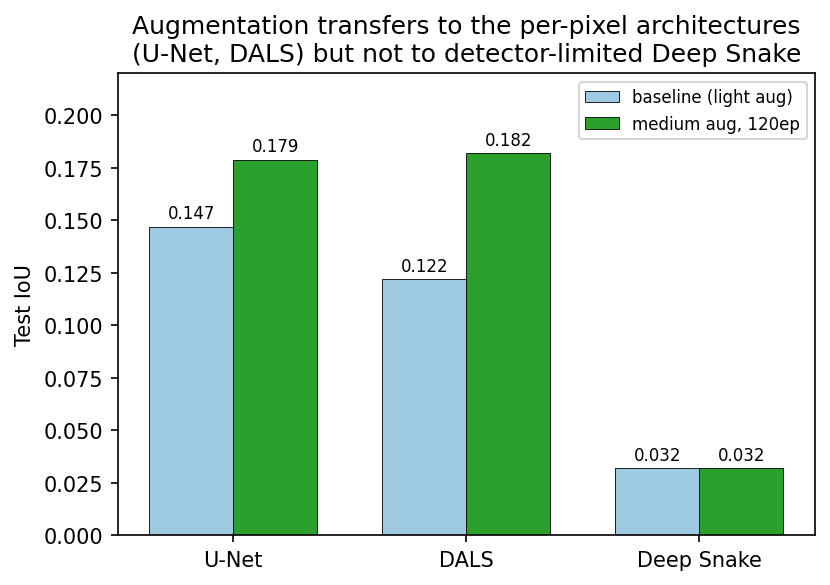
\includegraphics[width=0.58\textwidth]{figs/imp/transfer.png}
\caption{Augmentation transfer. The per-pixel architectures (U-Net, DALS) both
gain; the detector-limited Deep Snake is unchanged.}
\label{fig:transfer}
\end{figure}

\paragraph{A metric caveat: empty-GT frames and ``perfect'' IoU.} The IoU
convention scores an empty prediction against an empty GT as $1.0$ (both sets
empty $\Rightarrow$ perfect agreement). The deep eval, unlike the classical one,
does \emph{not} skip empty-GT frames---and the 94-frame test split contains
\textbf{3 frames whose thermal GT is empty} (no pixel $\ge150\,^\circ$C). It turns
out that \emph{every} IoU$=1.0$ in our results is one of these empty-on-empty
frames: \textbf{no frame containing actual fire was segmented perfectly by any
model}. Those 3 free $1.0$s inflate each reported mean by $\approx0.025$.
Table~\ref{tab:empty} restates the headline numbers on fire-containing frames
only ($n=91$).

\begin{table}[H]
\centering\small
\begin{tabular}{lrrr}
\toprule
Model & mean IoU (all 94) & mean IoU (GT$>$0, $n{=}91$) & \# IoU$=1$ (all empty-GT) \\
\midrule
U-Net + aug & 0.179 & 0.152 & 3 \\
\textbf{DALS + aug} & \textbf{0.182} & \textbf{0.155} & 3 \\
U-Net baseline & 0.147 & 0.130 & 2 \\
DALS baseline & 0.122 & 0.126 & 0 \\
Deep Snake + aug & 0.032 & \textbf{0.000} & 3 \\
\bottomrule
\end{tabular}
\caption{Empty-GT frames give free IoU$=1.0$. The ranking is unchanged and
DALS$+$aug remains best, but absolute scores drop $\sim$0.025 on real fire. Most
striking: \textbf{Deep Snake scores exactly 0.000 on fire-containing frames}---its
entire $0.032$ is the three empty freebies, confirming it detects no actual
fire.}
\label{tab:empty}
\end{table}

\begin{figure}[H]
\centering
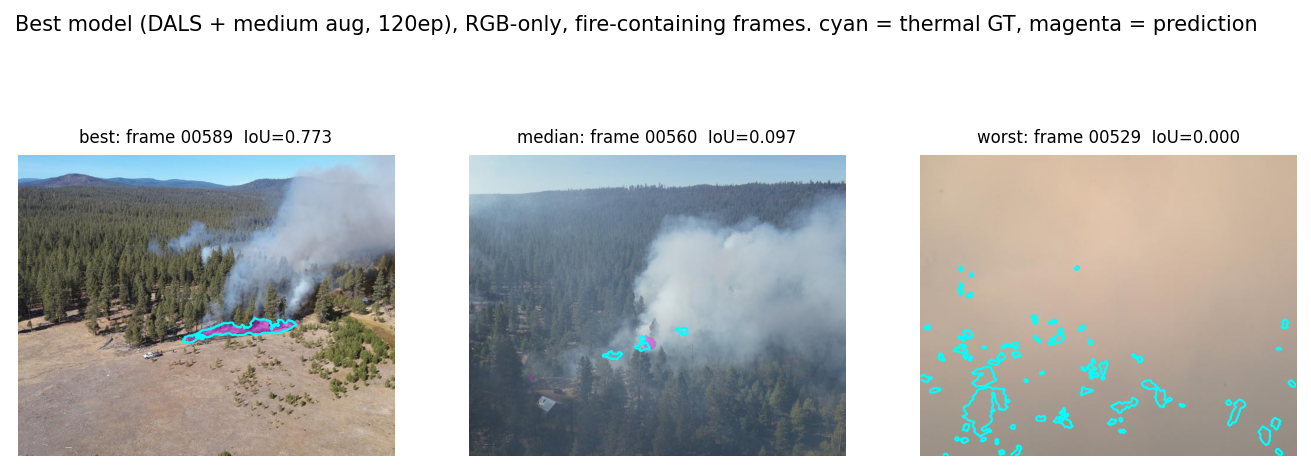
\includegraphics[width=\textwidth]{figs/imp/qual_aug2.png}
\caption{Best/median/worst test frames for the U-Net + medium aug (120ep) model,
RGB-only, no location prior. Cyan = thermal GT, magenta = prediction. (DALS + aug
scores marginally higher overall, 0.182.)}
\label{fig:qual}
\end{figure}

\section{Removing Degenerate (Fully-Occluded) Frames}

A natural data-cleaning step is to drop frames where smoke covers the
\emph{entire} image: there the fire location is unrecoverable from RGB by any
method, so they are degenerate inputs. We score each frame's smoke fraction
(bright $\cap$ desaturated $\cap$ low-texture pixels) and exclude those
$\ge0.95$---\textbf{32 of 622 frames} (Fig.~\ref{fig:removed}). Notably these
frames \emph{still contain thermal GT} (up to $\sim$10k hot pixels): the fire is
real, just invisible in RGB. Of the 32, 24 fall in train, 7 in val, 1 in test, so
filtering is mostly a \emph{training-set} cleanup; the test set barely changes
($94\!\to\!89$).

\begin{figure}[H]
\centering
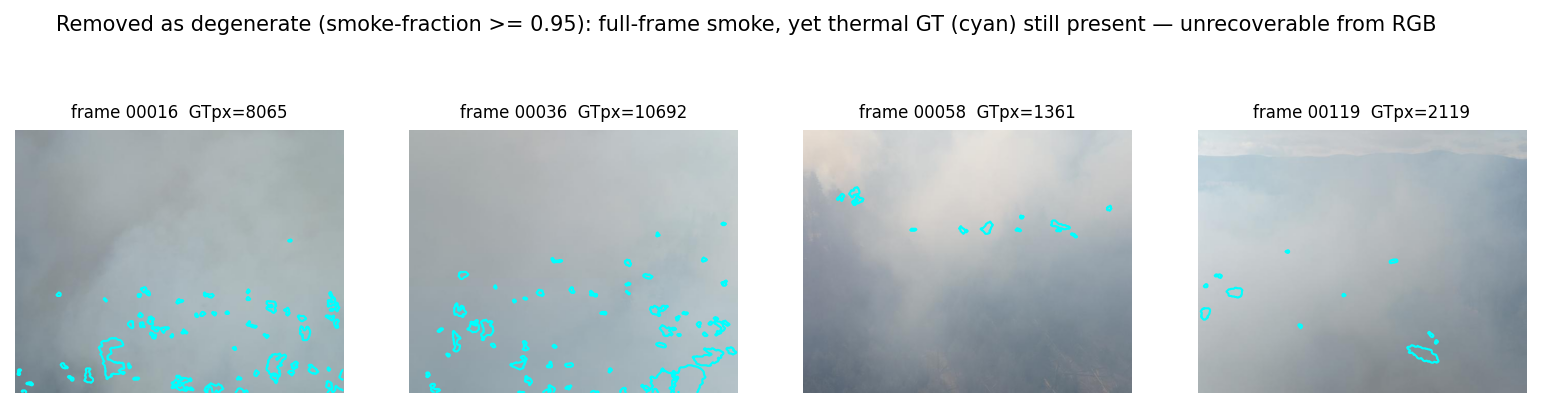
\includegraphics[width=\textwidth]{figs/imp/removed.png}
\caption{Four of the 32 removed frames. Full-frame smoke/haze, yet the thermal GT
(cyan) is substantial---unrecoverable from RGB, hence degenerate.}
\label{fig:removed}
\end{figure}

\paragraph{Effect, read honestly.} On the contaminated all-frames metric,
filtering appears to \emph{lower} the augmented models (DALS$+$aug
$0.182\!\to\!0.173$)---but that is the empty-GT artifact again: filtering drops
one empty-GT test frame, removing a free $1.0$. On the meaningful
\textbf{fire-only} metric (Fig.~\ref{fig:filter}), the picture is clear: filtering
\emph{helps the light-aug baselines} (U-Net $0.130\!\to\!0.144$, DALS
$0.126\!\to\!0.132$)---the occluded frames were noise the weak models could not
absorb---but is \emph{neutral for the augmented models} (U-Net$+$aug
$0.152\!\to\!0.153$, DALS$+$aug $0.155\!\to\!0.154$, both within noise), which
already cope with occlusion. The honest conclusion: filtering yields a cleaner,
better-defined task with the \emph{same} top performance; it does not raise the
best model's real-fire score. For the augmented models the data-starvation cost
of $-24$ training frames roughly cancels the noise-reduction benefit.

\begin{figure}[H]
\centering
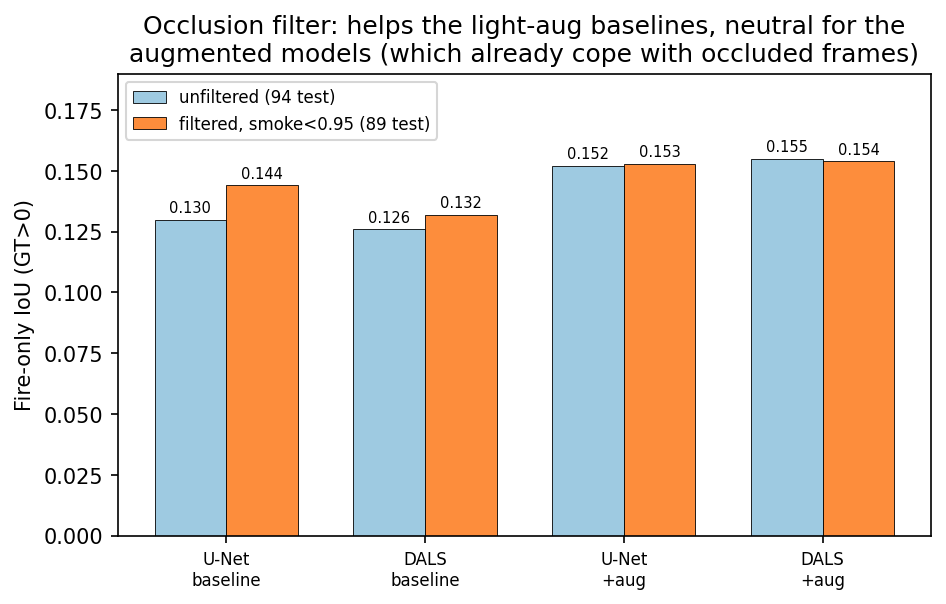
\includegraphics[width=0.62\textwidth]{figs/imp/filter.png}
\caption{Fire-only IoU, unfiltered vs.\ filtered. Filtering helps the baselines,
is neutral for the augmented models.}
\label{fig:filter}
\end{figure}

\section{Conclusions}

\textbf{1. The task is data-limited, not information-limited.} The learning curve
is the key evidence: val IoU rises with data and has not plateaued. The signal
exists in the RGB; we lack the labelled frames to exploit it from scratch.

\textbf{2. Only interventions that add information move the needle.} Loss
reweighting, engineered channels, contour refinement, and a richer output target
were all flat or negative---they operate on information already available.
Augmentation (synthetic data) is the first to help, and it helps precisely
because it attacks the confirmed bottleneck.

\textbf{3. The fix generalises to architectures that can use the data.}
Medium augmentation lifts both per-pixel architectures (U-Net $+22\%$, DALS
$+49\%$) but leaves Deep Snake unchanged---its bottleneck is contour
\emph{seeding}, not data. That augmentation helps exactly the architectures whose
limit is sample count, and only those, is independent confirmation of the
data-starvation diagnosis.

\textbf{4. Removing degenerate frames cleans the task without raising the
ceiling.} Excluding the 32 full-frame-smoke inputs helps the weak baselines
(noise removal) but is neutral for the augmented models, whose augmentation
already absorbs the occlusion. The benefit and the data-starvation cost cancel;
the value is a better-defined benchmark, not a higher score.

\textbf{5. Negative results require controlled tests.} The first augmentation run
``failed'' only because of a convergence confound; the first regularisation
sweep looked like ``no signal'' only because none of the levers added any. Both
near-conclusions were corrected by a more careful experiment---a reminder that an
underpowered or confounded run can masquerade as a scientific result.

\textbf{6. Best prior-free detector: DALS + medium augmentation}, fire-only IoU
$\approx0.155$ (all-frames 0.182; U-Net + aug close behind), $+49\%$ over the DALS
baseline and roughly halving the gap to oracle-GAC \emph{without} any location
prior---on either the full or the occlusion-filtered test set. Note no model
perfectly segments any fire-containing frame; every IoU$=1.0$ is an empty-on-empty
test frame, a metric artifact we report transparently (Table~\ref{tab:empty}).

\paragraph{Next steps.} The data-starvation diagnosis points to information-adding
levers we have not yet tried: an \textbf{ImageNet-pretrained backbone} (borrows
millions of images of external data---the strongest remaining fix), stacking the
proven augmentation with Focal-Tversky, and ingesting more FLAME-3 frames. A
combined run was deferred to keep causal attribution clean.

\end{document}
